%% -*- coding: utf-8 -*-
\documentclass[12pt,a4paper]{scrartcl} 
\usepackage[utf8]{inputenc}
\usepackage[english,russian]{babel}
\usepackage{indentfirst}
\usepackage{misccorr}
\usepackage{graphicx}
\usepackage{amsmath}
\begin{document}
	\begin{titlepage}
		\begin{center}
			\large
			МИНИСТЕРСТВО НАУКИ И ВЫСШЕГО ОБРАЗОВАНИЯ РОССИЙСКОЙ ФЕДЕРАЦИИ
			
			Федеральное государственное бюджетное образовательное учреждение высшего образования
			
			\textbf{АДЫГЕЙСКИЙ ГОСУДАРСТВЕННЫЙ УНИВЕРСИТЕТ}
			\vspace{0.25cm}
			
			Инженерно-физический факультет
			
			Кафедра автоматизированных систем обработки информации и управления
			\vfill

			\vfill
			
			\textsc{Отчет по практике}\\[5mm]
			
			{\LARGE \textit{Сортировки Быстрая и Слиянием}}
			\bigskip
			
			2 курс, группа 2УТС
		\end{center}
		\vfill
		
		\newlength{\ML}
		\settowidth{\ML}{«\underline{\hspace{0.7cm}}» \underline{\hspace{2cm}}}
		\hfill\begin{minipage}{0.5\textwidth}
			Выполнил:\\
			\underline{\hspace{\ML}} В.\,В.~Пащенко\\
			«\underline{\hspace{0.7cm}}» \underline{\hspace{2cm}} 2022 г.
		\end{minipage}%
		\bigskip
		
		\hfill\begin{minipage}{0.5\textwidth}
			Руководитель:\\
			\underline{\hspace{\ML}} С.\,В.~Теплоухов\\
			«\underline{\hspace{0.7cm}}» \underline{\hspace{2cm}} 2022 г.
		\end{minipage}%
		\vfill
		
		\begin{center}
			Майкоп, 2022 г.
		\end{center}
	\end{titlepage}
		
	\section{Введение}
	\label{sec:intro}
	\begin{enumerate}
	\item Текстовая формулировка задачи:
	
	Написать программу для сортировки массива быстрым алгоритмом и слиянием.
	\item Пример программного кода, решающего данную задачу на языке C++, приведен в пункте~\ref{sec:exp:code} на стр.~\pageref{sec:exp:code}.
	\item Результаты работы программы представлены в пункте~\ref{sec:result:screen} на стр.~\pageref{figure1:screen} и~\pageref{figure2:screen}.
	\end{enumerate}
	
	\section{Ход работы}
	\label{sec:exp}
	
	\subsection{Код программы}
	\label{sec:exp:code}
	\begin{verbatim}
	#include <iostream>
	#include <locale>
	using namespace std;
	
	// Быстрая сортировка
	int section(int mas[], int start, int end)
	{
	    int point = mas[start];
	    int count = 0;
	    for (int i = start + 1; i <= end; i++)
	    {
	        if (mas[i] <= point)
	            count++;
	    }
	    // Придание поворотному элементу правильного положения
	    int index = start + count;
	    swap(mas[index], mas[start]);
	    // Сортировка левой и правой частей поворотного элемента
	    int i = start, j = end;
	    while (i < index && j > index)
	    {
	        while (mas[i] <= point)
	            i++;
	        while (mas[j] > point)
	            j--;
	        if (i < index && j > index)
	            swap(mas[i++], mas[j--]);
	    }
	    return index;
	}
	void sortirovka(int mas[], int start, int end)
	{
	    // базовый корпус
	    if (start >= end)
	        return;
	    // разбиение массива на разделы
	    int p = section(mas, start, end);
	    // Сортировка левой части
	    sortirovka(mas, start, p - 1);
	    // Сортировка правой части
	    sortirovka(mas, p + 1, end);
	}
	
	// Сортировка слиянием
	void sort(int*, int, int, int);
	void _sortirovka_(int* arr, int low, int high)
	{
	    int mid;
	    if (low < high)
	    {
	        mid = (low + high) / 2;
	        _sortirovka_(arr, low, mid);
	        _sortirovka_(arr, mid + 1, high);
	        sort(arr, low, high, mid);
	    }
	}
	void sort(int* arr, int low, int high, int mid)
	{
	    int i, j, k, c[50];
	    i = low;
	    k = low;
	    j = mid + 1;
	    while (i <= mid && j <= high)
	    {
	        if (arr[i] < arr[j])
	        {
	            c[k] = arr[i];
	            k++;
	            i++;
	        }
	        else
	        {
	            c[k] = arr[j];
	            k++;
	            j++;
	        }
	    }
	    while (i <= mid)
	    {
	        c[k] = arr[i];
	        k++;
	        i++;
	    }
	    while (j <= high)
	    {
	        c[k] = arr[j];
	        k++;
	        j++;
	    }
	    for (i = low; i < k; i++)
	        arr[i] = c[i];
	}
	
	int main()
	{
	    setlocale(LC_ALL, "rus");
	    int n;
	    do
	    {
	        cout << "Введите размерность массива: ";
	        cin >> n;
	        if (n <= 0)
	            cout << "Ошибка" << endl;
	    }
	    while (n <= 0);
	
	    int mas[100];
	    cout << "Введите массив: ";
	    for (int i = 0; i < n; i++)
	        cin >> mas[i];
	    int vibor;
	
	    do
	    {
	        cout << endl << "1 - быстрая сортировка" << endl
			  <<  "2 - сортировка слиянием" << endl << "Выберите способ сортировки: ";
	        cin >> vibor;
	        if (vibor != 1 && vibor != 2)
	            cout << "Ошибка" << endl;
	    }
	    while (vibor != 1 && vibor != 2);
	    
	    switch (vibor)
	    {
	        case 1:
	            sortirovka(mas, 0, n - 1);
	            cout << "Отсортированный массив: ";
	            for (int i = 0; i < n; i++)
	                cout << mas[i] << " ";
	            break;
	        case 2:
	            _sortirovka_(mas, 0, n - 1);
	            cout << "Отсортированный массив: ";
	            for (int i = 0; i < n; i++)
	                cout << mas[i] << " ";
	            break;
	    }
	}	
	\end{verbatim}
	
	\section{Результат работы программы}
	\label{sec:result}
	
	\subsection{Скриншоты выполнения кода}
	\label{sec:result:screen}
	\begin{figure}[h]
	\centering
	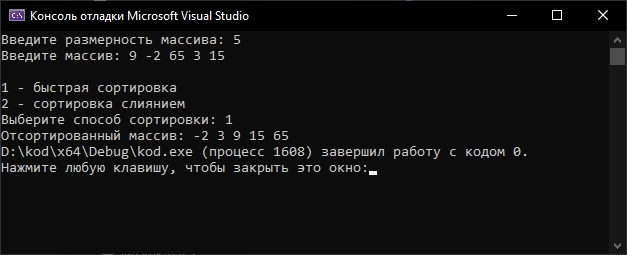
\includegraphics[width=1\textwidth]{res1.jpg}
	\caption{Быстрая сортировка}\label{figure1:screen}
	\end{figure}

	\begin{figure}[h]
	\centering
	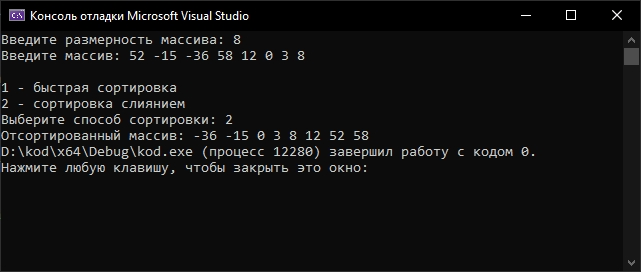
\includegraphics[width=1\textwidth]{res2.jpg}
	\caption{Cортировка слиянием}\label{figure2:screen}
	\end{figure}

	\begin{thebibliography}{9}
	\bibitem{Knuth-2003}Кнут Д.Э. Всё про \TeX. \newblock --- Москва: Изд. Вильямс, 2003 г. 550~с.
	\bibitem{Lvovsky-2003}Львовский С.М. Набор и верстка в системе \LaTeX{}. \newblock --- 3-е издание, исправленное и дополненное, 2003 г.
	\bibitem{Voroncov-2005}Воронцов К.В. \LaTeX{} в примерах. 2005 г.
	\bibitem{Stroustrup-2011_1}Страуструп, Бьерн. Программирование. Принципы и практика использования C++ / Бьярне Страуструп ; [пер. с англ. и ред. Д. А. Клюшина]. - Москва [и др.] : Вильямс, 2011. - 1238 с. : ил., табл.; 24 см.
	\bibitem{Stroustrup-2011_2}Страуструп, Бьерн. Язык программирования C++ / Бьерн Страуструп ; пер. с англ. под ред. Н. Н. Мартынова. - Спец. изд. - Москва : Бином, 2011. - 1135 с. : ил.; 24 см.

	\end{thebibliography}
	
\end{document}
